\documentclass[dvips,12pt]{article}

% Any percent sign marks a comment to the end of the line

% Every latex document starts with a documentclass declaration like this
% The option dvips allows for graphics, 12pt is the font size, and article
%   is the style

\usepackage[pdftex]{graphicx}
\usepackage{url}
\usepackage{graphicx}
\usepackage{subcaption}



% These are additional packages for "pdflatex", graphics, and to include
% hyperlinks inside a document.

\setlength{\oddsidemargin}{0.25in}
\setlength{\textwidth}{6.5in}
\setlength{\topmargin}{0in}
\setlength{\textheight}{8.5in}

% These force using more of the margins that is the default style

\begin{document}

\title{Application Server Load Testing}
\author{Sharath Rao, Yuesong Wang, Ethan Preble, Mathieu Rodrigue}
\date{\today}

\maketitle

%20151111-2115 -- m3.medium
%2151 -- m3.large
%2320 -- m3.xlarge
%

\section{Tsung Load Testing}

In this section, we describe the results from load testing with both vertically and horizontally scaled application servers.

\subsection{Vertical Scaling}

Vertical scaling was tested in 6 phases with 2, 4, 8, 16, 32, and 64 users arriving at the page every second.

\subsubsection{Observations}

\begin{itemize}
  \item Our first request takes a long time to load as many users come to visit the site.
  \item Increasing server size does not seem to do much for average transaction times.
  \item The number of 500 and 503 status codes reduced as the servers increased in performance, allowing to serve more users
  \item The number of 200 status codes increased proportionally as 500 and 503 decreased.
  \item The number of connected users increases as we increase server performance.
\end{itemize}
\newpage

\begin{figure}[h!]
    \centering
    \begin{subfigure}[b]{0.3\textwidth}
        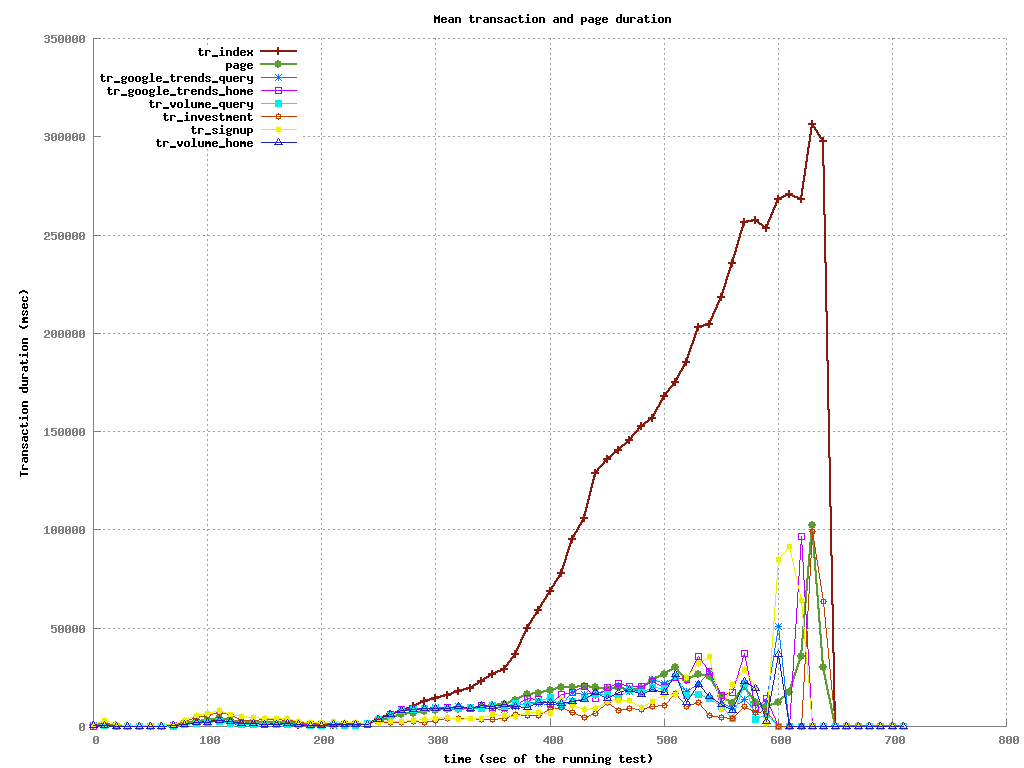
\includegraphics[width=\textwidth]{images/vertical/transaction_medium.png}
        \caption{m3.medium}
    \end{subfigure}
    ~ 
    \begin{subfigure}[b]{0.3\textwidth}
        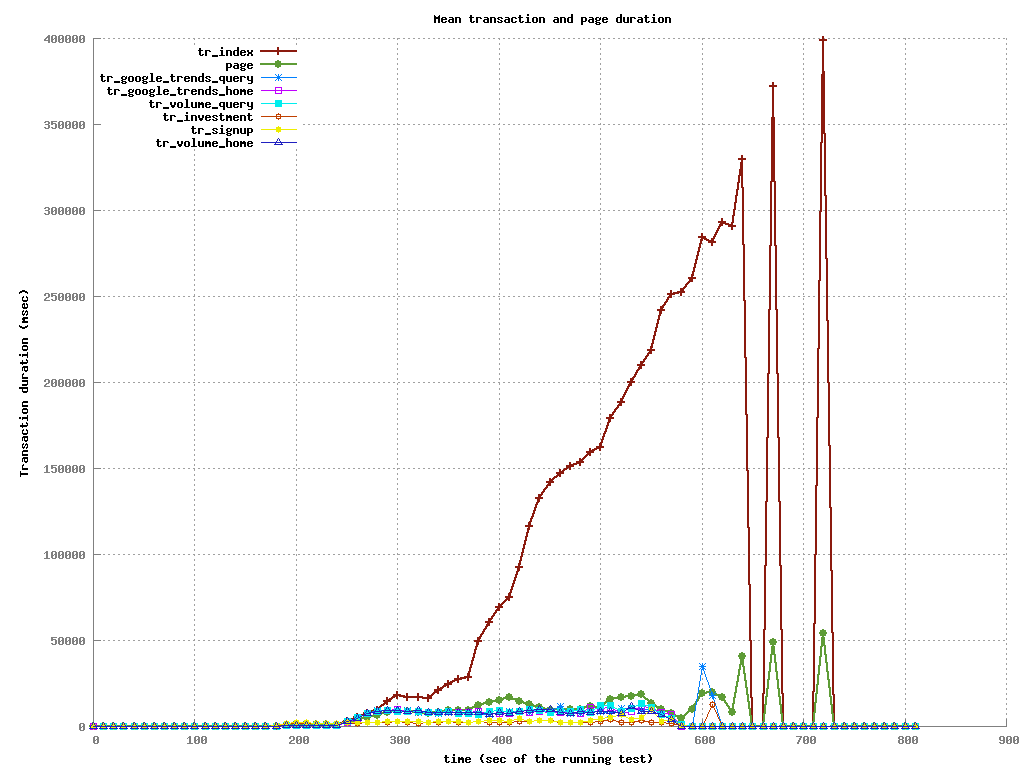
\includegraphics[width=\textwidth]{images/vertical/transaction_large.png}
        \caption{m3.large}
    \end{subfigure}
    ~ 
    \begin{subfigure}[b]{0.3\textwidth}
        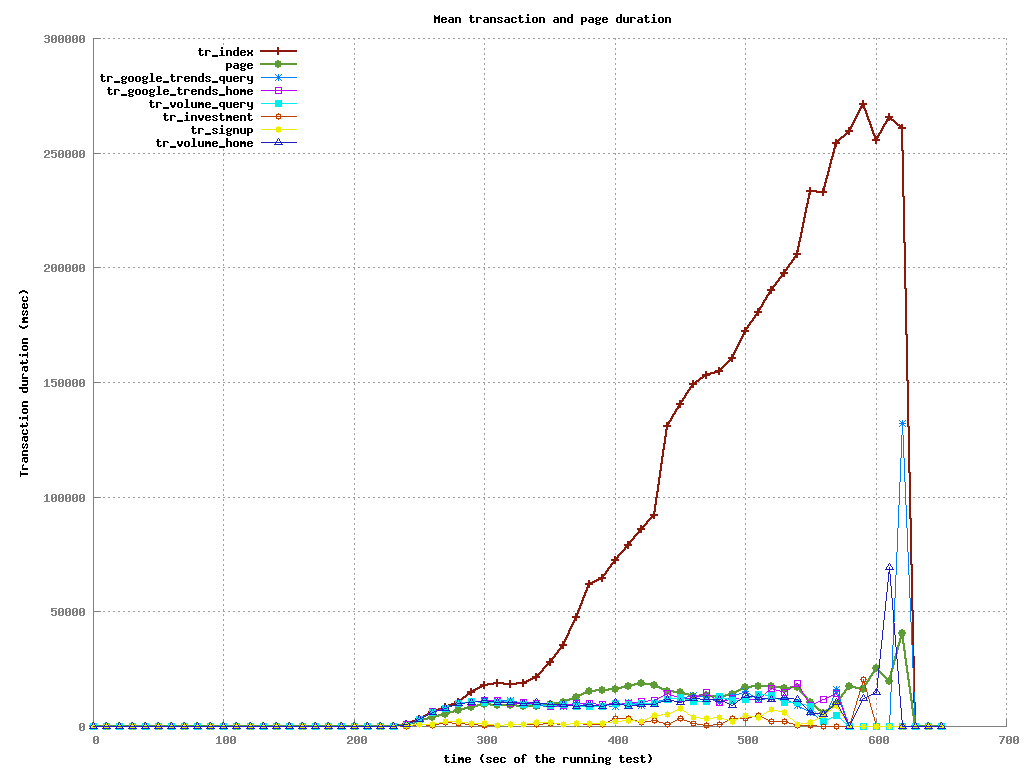
\includegraphics[width=\textwidth]{images/vertical/transaction_xlarge.png}
        \caption{m3.xlarge}
    \end{subfigure}
    \caption{Mean transaction and page duration for three m3 instances.}
\end{figure}

\begin{figure}[h!]
    \centering
    \begin{subfigure}[b]{0.3\textwidth}
        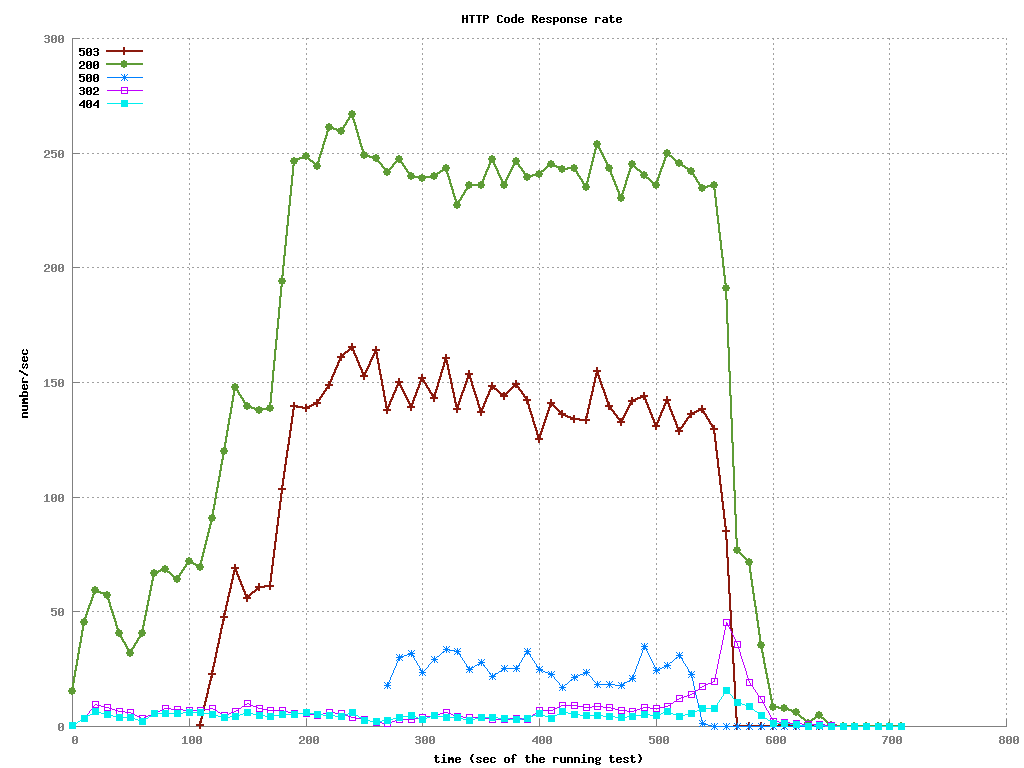
\includegraphics[width=\textwidth]{images/vertical/http_code_medium.png}
        \caption{m3.medium}
    \end{subfigure}
    ~ 
    \begin{subfigure}[b]{0.3\textwidth}
        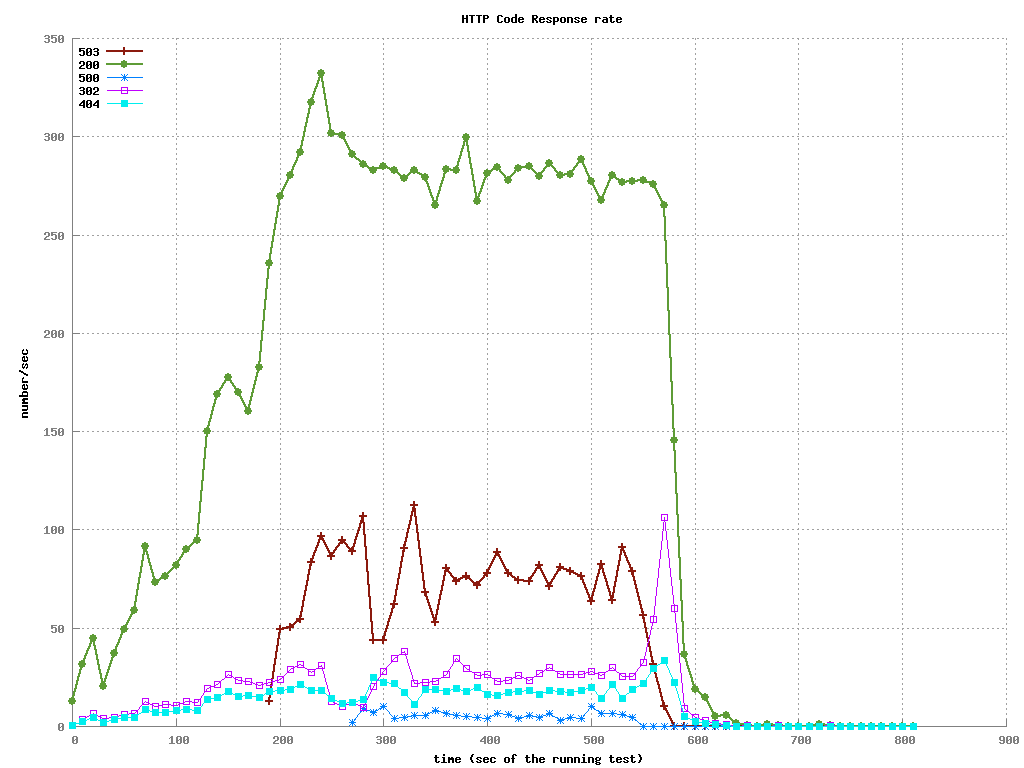
\includegraphics[width=\textwidth]{images/vertical/http_code_large.png}
        \caption{m3.large}
    \end{subfigure}
    ~ 
    \begin{subfigure}[b]{0.3\textwidth}
        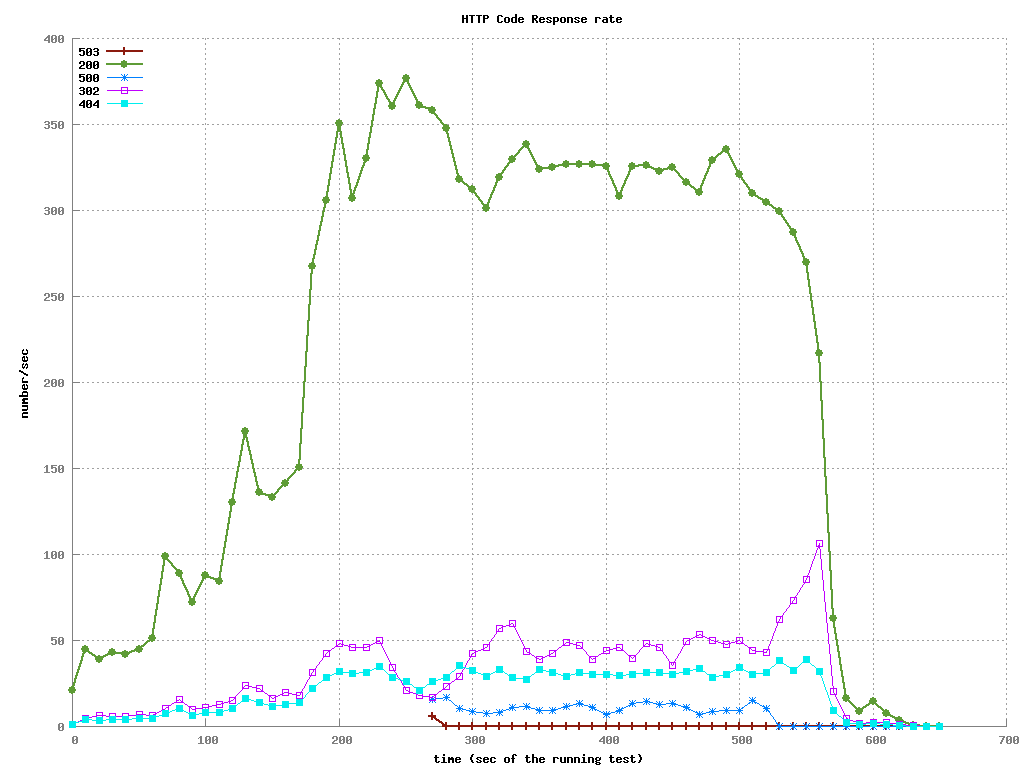
\includegraphics[width=\textwidth]{images/vertical/http_code_xlarge.png}
        \caption{m3.xlarge}
    \end{subfigure}
    \caption{HTTP code rate for three m3 instances.}
\end{figure}

\begin{figure}[h!]
    \centering
    \begin{subfigure}[b]{0.3\textwidth}
        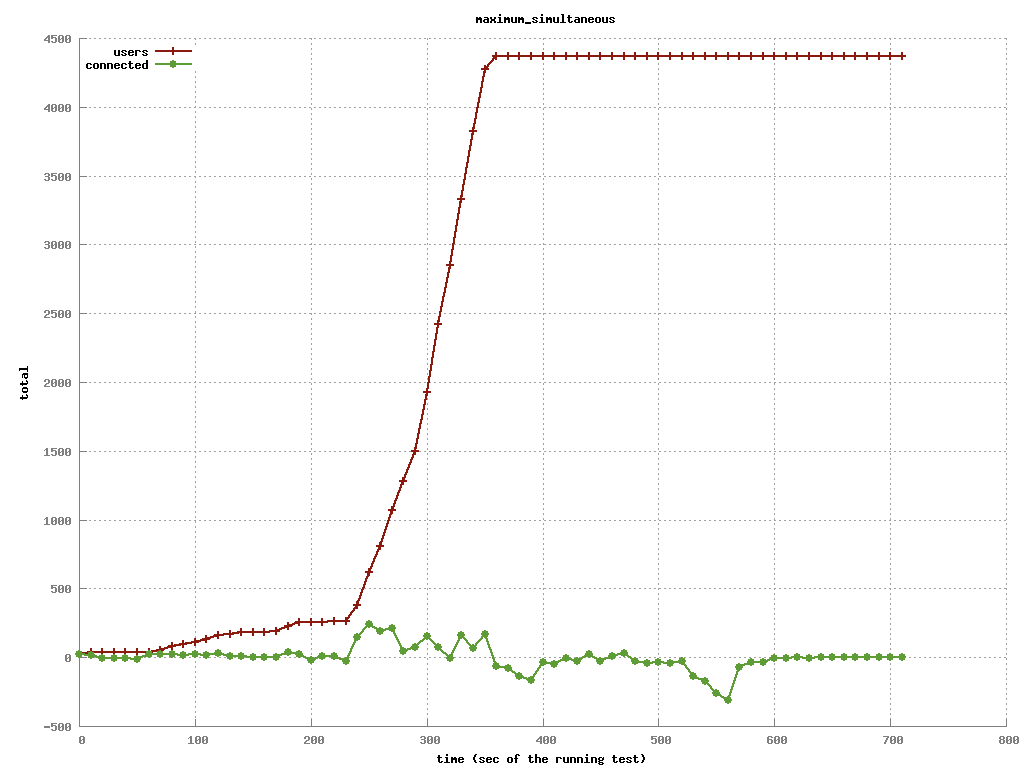
\includegraphics[width=\textwidth]{images/vertical/users_simul_medium.png}
        \caption{m3.medium}
    \end{subfigure}
    ~ 
    \begin{subfigure}[b]{0.3\textwidth}
        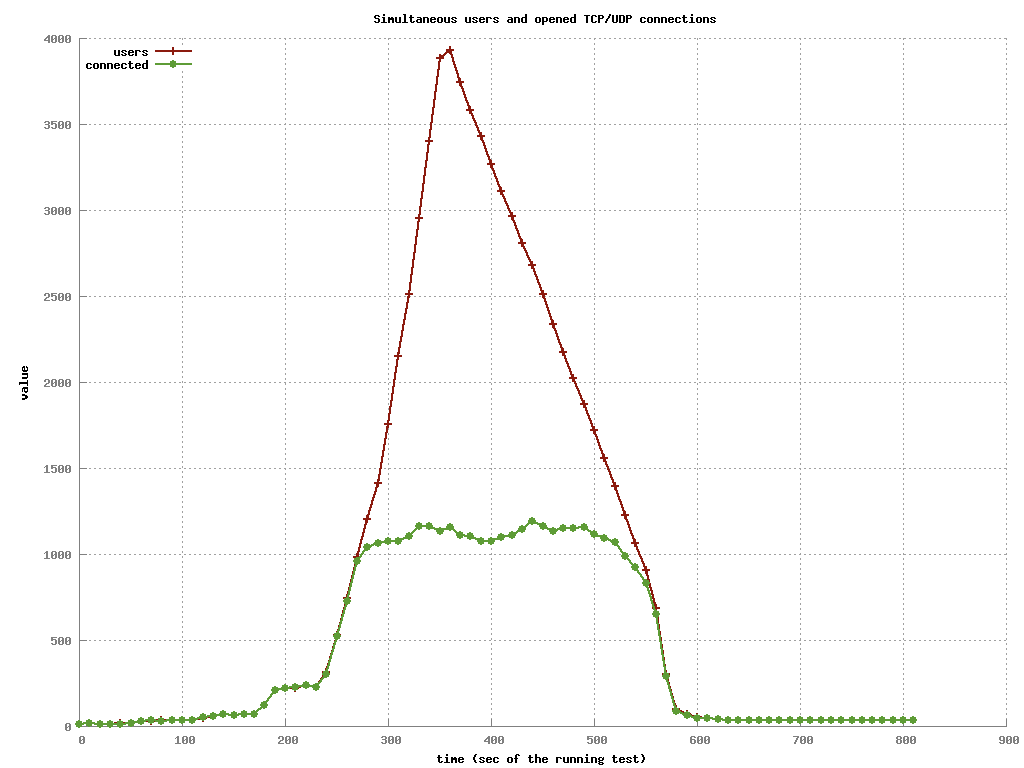
\includegraphics[width=\textwidth]{images/vertical/users_simul_large.png}
        \caption{m3.large}
    \end{subfigure}
    ~ 
    \begin{subfigure}[b]{0.3\textwidth}
        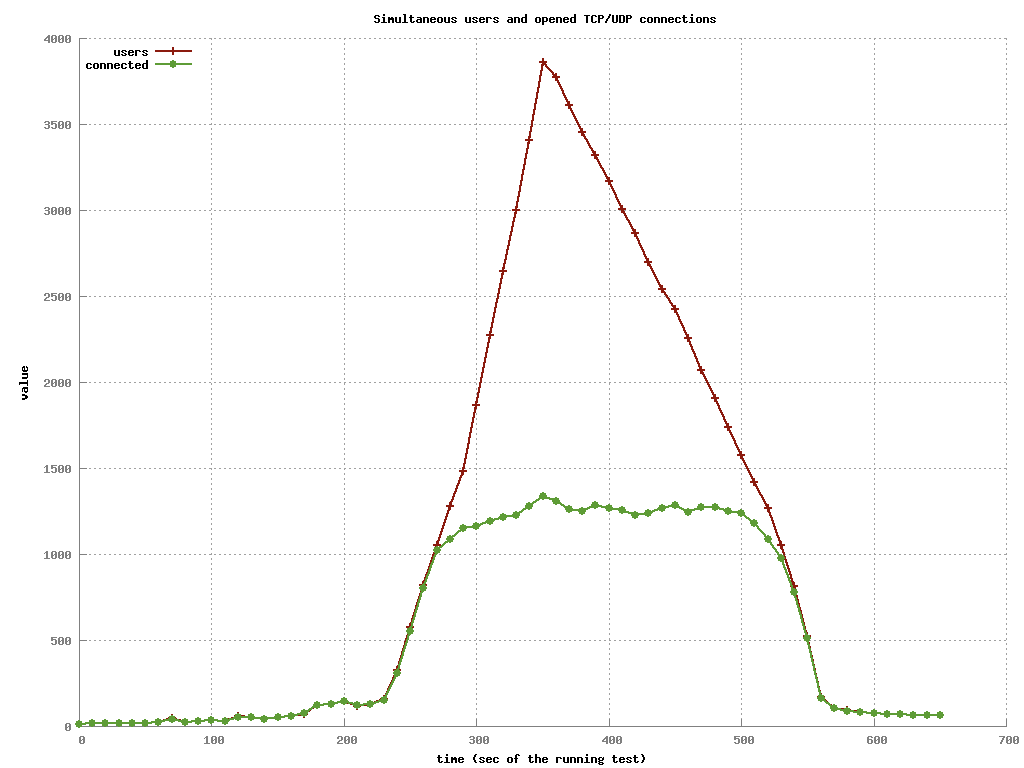
\includegraphics[width=\textwidth]{images/vertical/users_simul_xlarge.png}
        \caption{m3.xlarge}
    \end{subfigure}
    \caption{Number of simultaneous users for three m3 instances.}
\end{figure}



%\begin{figure}
%\begin{center}
%\resizebox{6in}{!}{\includegraphics*{graphimage.jpg}}
%\end{center}

%\caption{image caption}
%
%\end{figure}

\newpage
\subsection{Horizontal Scaling}

This section will discuss horizontal scaling

\newpage
\begin{figure}[h!]
    \centering
    \begin{subfigure}[b]{0.3\textwidth}
        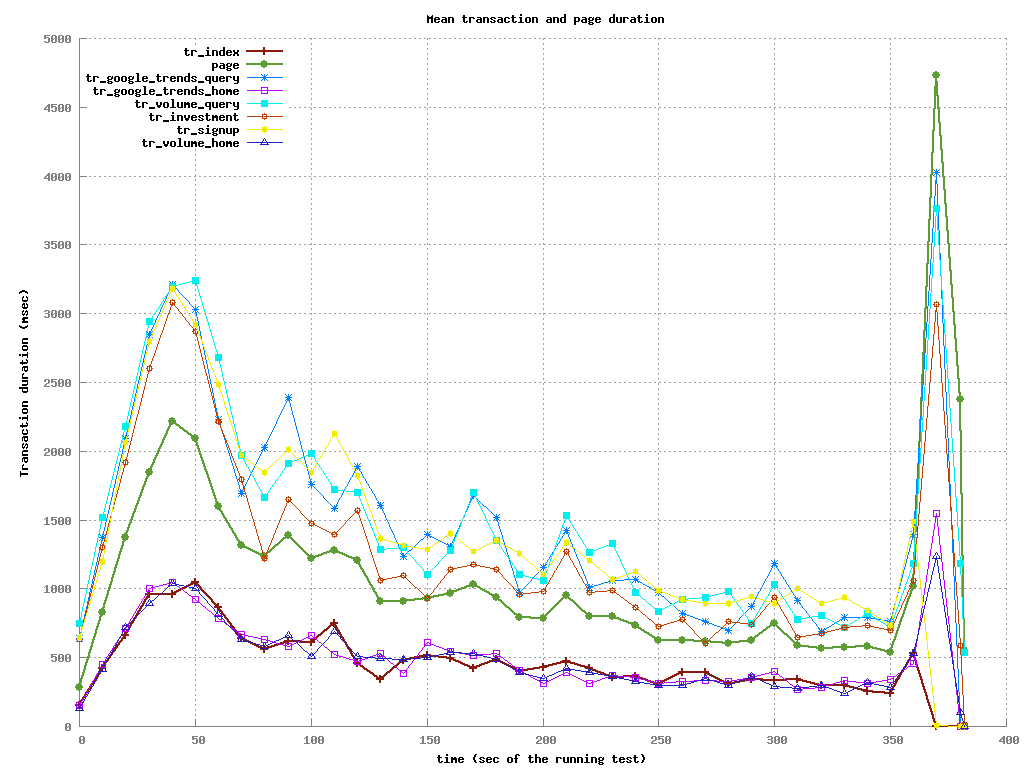
\includegraphics[width=\textwidth]{images/horizontal_m3large_dbm3large/transaction_1.png}
        \caption{One instance}
    \end{subfigure}
    ~ 
    \begin{subfigure}[b]{0.3\textwidth}
        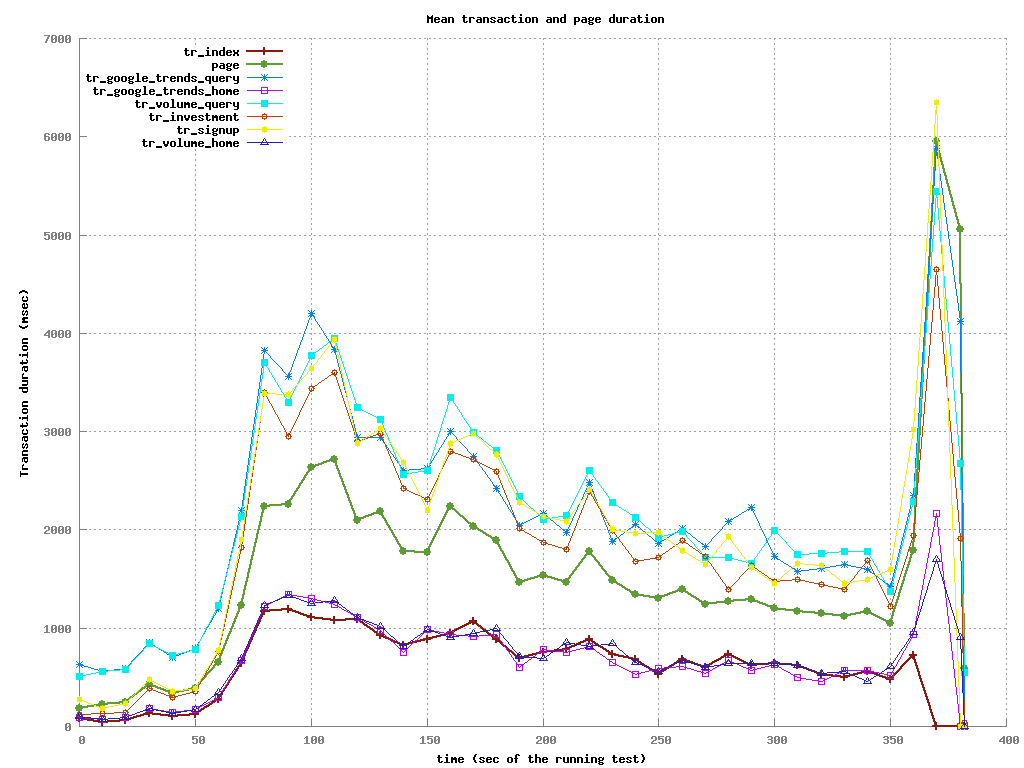
\includegraphics[width=\textwidth]{images/horizontal_m3large_dbm3large/transaction_2.png}
        \caption{Two instances}
    \end{subfigure}
    ~ 
    \begin{subfigure}[b]{0.3\textwidth}
        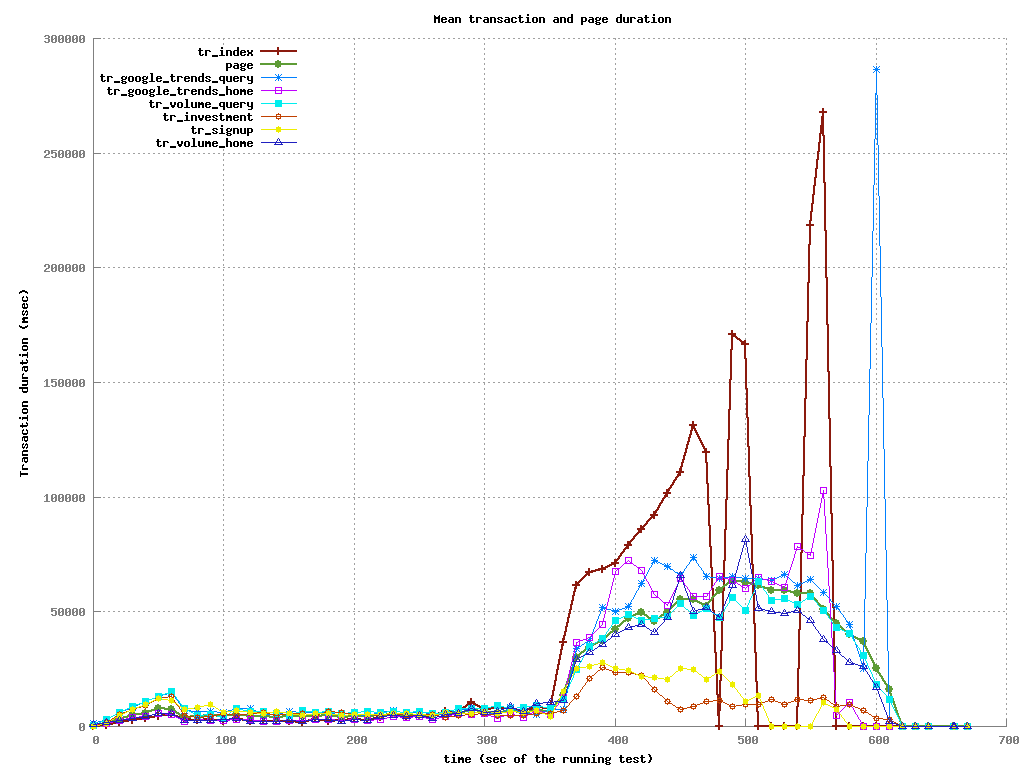
\includegraphics[width=\textwidth]{images/horizontal_m3large_dbm3large/transaction_4.png}
        \caption{Three instances}
    \end{subfigure}
    \caption{Mean transaction and page duration for m3.large instances.}
\end{figure}

\begin{figure}[h!]
    \centering
    \begin{subfigure}[b]{0.3\textwidth}
        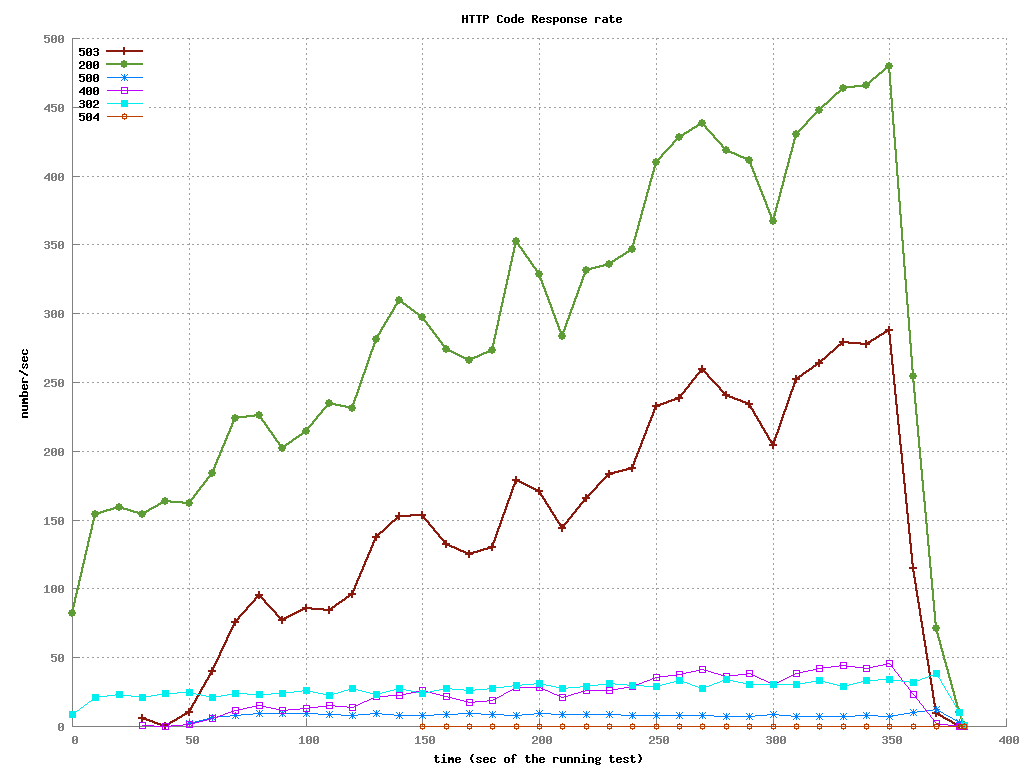
\includegraphics[width=\textwidth]{images/horizontal_m3large_dbm3large/http_1.png}
        \caption{Once instance}
    \end{subfigure}
    ~ 
    \begin{subfigure}[b]{0.3\textwidth}
        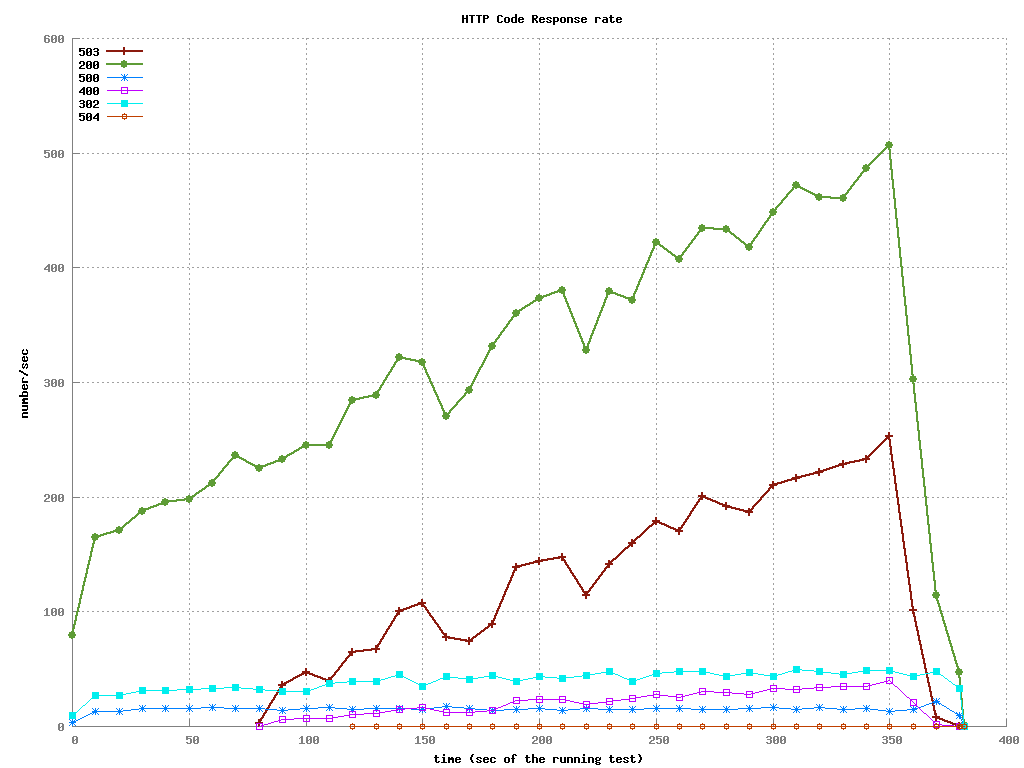
\includegraphics[width=\textwidth]{images/horizontal_m3large_dbm3large/http_2.png}
        \caption{Two instances}
    \end{subfigure}
    ~ 
    \begin{subfigure}[b]{0.3\textwidth}
        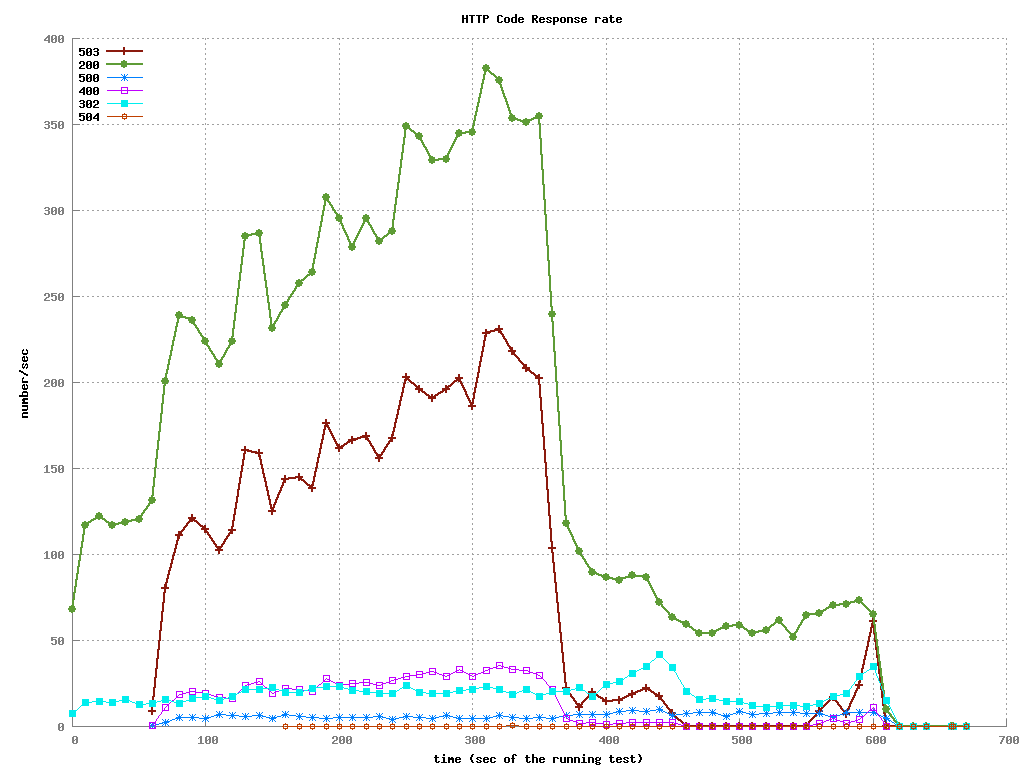
\includegraphics[width=\textwidth]{images/horizontal_m3large_dbm3large/http_4.png}
        \caption{Three instances}
    \end{subfigure}
    \caption{HTTP code rate for m3.large instances.}
\end{figure}

\begin{figure}[h!]
    \centering
    \begin{subfigure}[b]{0.3\textwidth}
        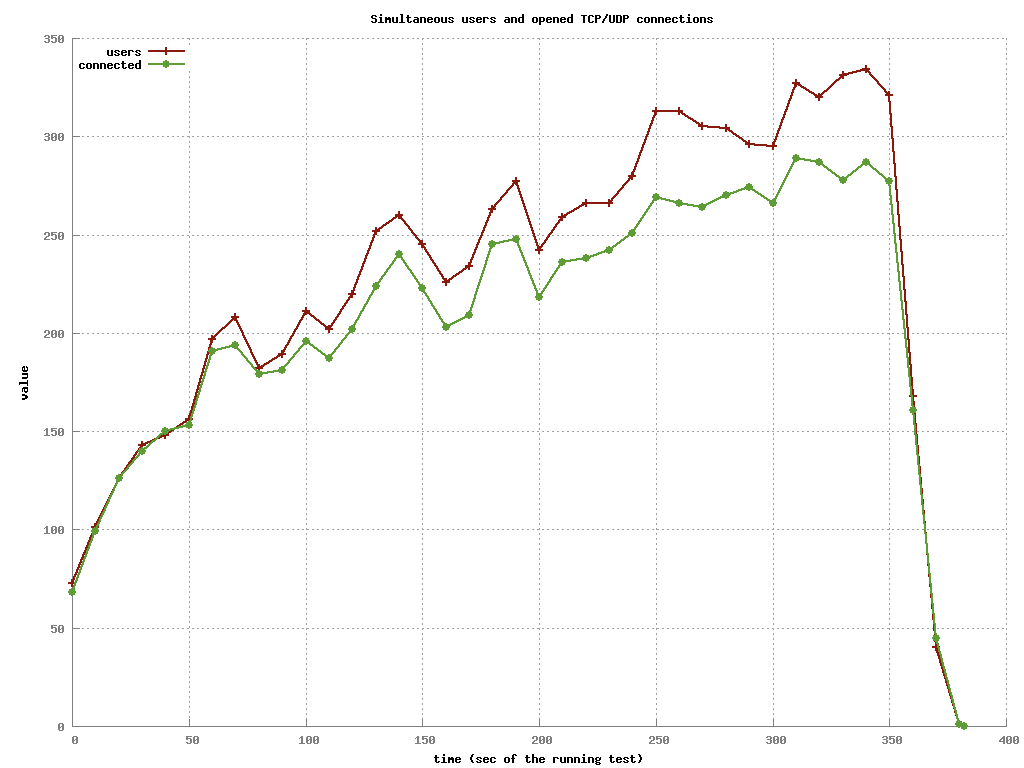
\includegraphics[width=\textwidth]{images/horizontal_m3large_dbm3large/sim_users_1.png}
        \caption{One instance}
    \end{subfigure}
    ~ 
    \begin{subfigure}[b]{0.3\textwidth}
        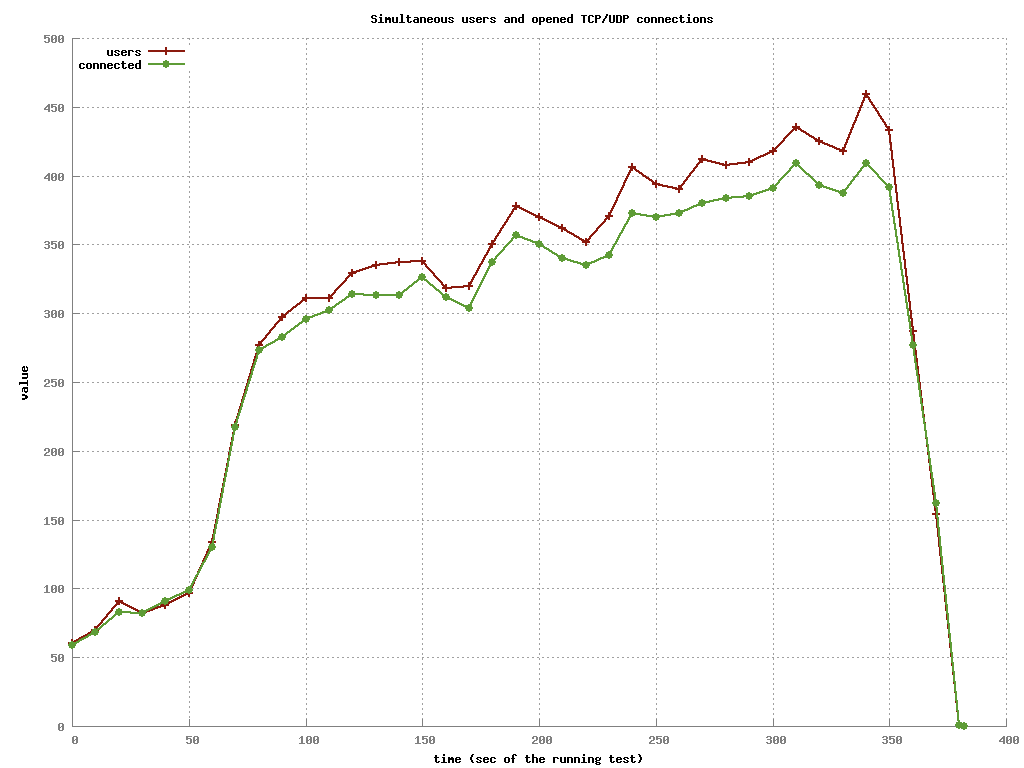
\includegraphics[width=\textwidth]{images/horizontal_m3large_dbm3large/sim_users_2.png}
        \caption{Two instances}
    \end{subfigure}
    ~ 
    \begin{subfigure}[b]{0.3\textwidth}
        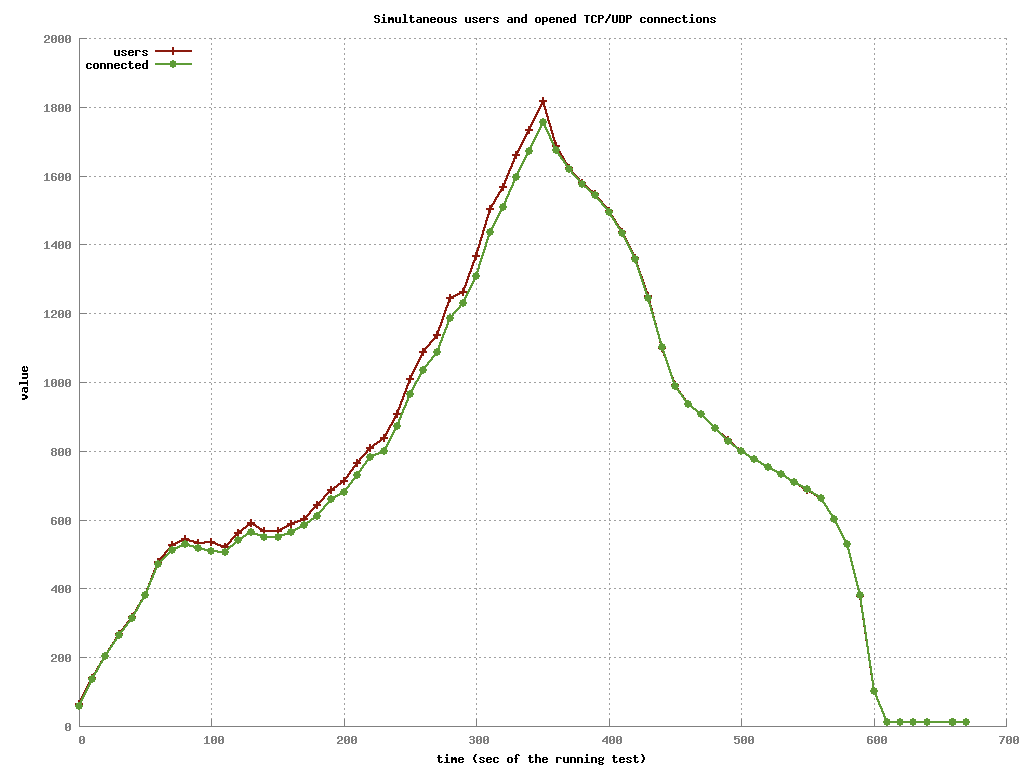
\includegraphics[width=\textwidth]{images/horizontal_m3large_dbm3large/sim_users_4.png}
        \caption{Three instances}
    \end{subfigure}
    \caption{Number of simultaneous users for m3.large instances.}
\end{figure}

\end{document}